%------------------------------------------------------------
% Introduction
\section{Introduction}
\label{sec:intro}

\begin{frame}{\nameref{sec:intro}: Bayesian inference}
    Let $Y$ and $\theta$ be a pair of random variables  with joint probability distribution $p(Y,\theta)$. With $\theta$ being the parameter of interest and $y$ the observed data, Bayes' rule is defined as follows:\footcite[pp.~6~f.]{gelman_bayesian_2013}

    \begin{block}{Bayes' rule}
        \begin{align}
            p(\theta|y) = \frac{p(y,\theta)}{p(y)} = \frac{p(y|\theta)p(\theta)}{p(y)}
        \end{align}
    \end{block}

    $p(y)$ with respect to $\theta$ is only a normalizing constant and can be ignored for inference such that one can write:
    \[\overbrace{p(\theta|y)}^\text{Posterior} \propto \overbrace{p(y|\theta)}^\text{Likelihood} \overbrace{p(\theta)}^\text{Prior}\]
\end{frame}

\begin{frame}{\nameref{sec:intro}: Shrinkage and sparsity}
    \begin{itemize}
        \item Shrinkage is a form of regularization where model parameters are shrunk towards zero
              \begin{itemize}
                  \item Example: Ridge regression\footcite{hoerl_ridge_2000} (L2 penalization)
                  \item $\text{arg} \min_{\beta} \left[ (y - X\beta)^T (y - X\beta) + \alpha \sum_{j = 1}^{p}\beta_j^2 \right]$
              \end{itemize}
        \item Sparsity refers to shrinking model parameters to exactly zero and therefore is a form of parameter selection
              \begin{itemize}
                  \item Example: Lasso regression\footcite{tibshirani_regression_1996} (L1 penalization)
                  \item $\text{arg} \min_{\beta} \left[ (y - X\beta)^T (y - X\beta) + \lambda \sum_{j = 1}^{p}|\beta_j| \right]$
              \end{itemize}
    \end{itemize}~\\
    
    Sparsity and/or shrinkage in Bayesian modeling can be realized through the choice of a prior distribution.
    \begin{itemize}
        \item Example: A regression model with a Laplace prior centered at zero is the Bayesian counterpart to a Lasso regression (proof in \nameref{sec:appendix})
    \end{itemize}
\end{frame}

\begin{frame}{\nameref{sec:intro}: Lasso example\footnote{Source code: \url{https://github.com/phipag/r-lasso-bayesian}}$^\text{,}$\footnote{Data description: \url{https://tinyurl.com/rmtcars}} I}
    \begin{figure}
        \centering
        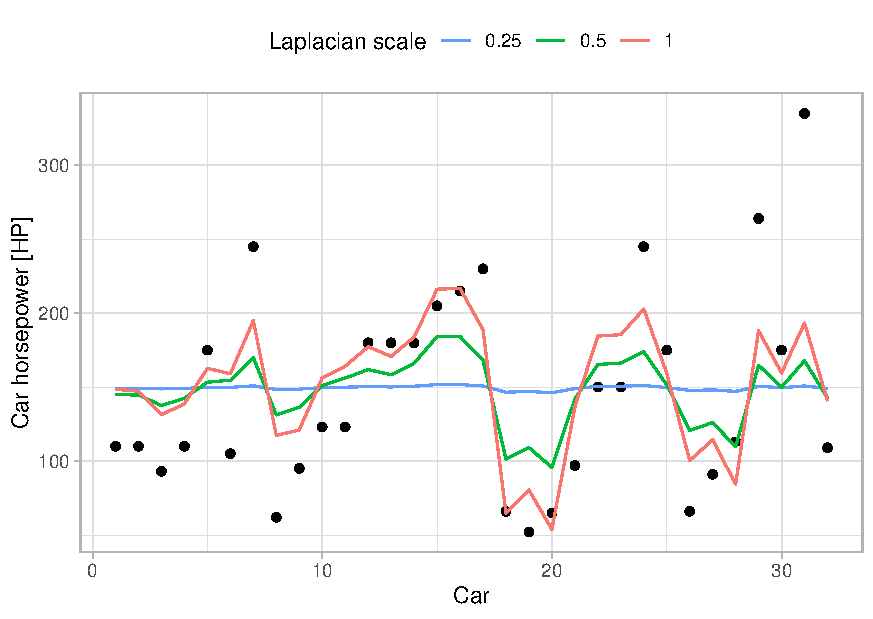
\includegraphics[width=\textwidth,height=.65\textheight,keepaspectratio]{plots/bayesian_lasso_fit.pdf}
        \caption{Bayesian Lasso model fit}
        \label{fig:bayesian_lasso_fit}
    \end{figure}
\end{frame}

\begin{frame}{\nameref{sec:intro}: Lasso example II}
    \begin{figure}
        \centering
        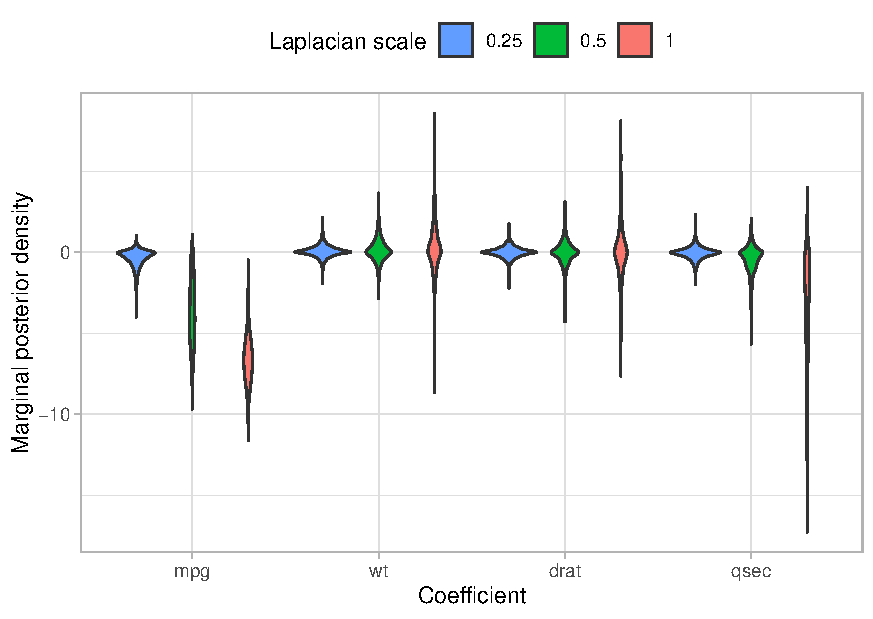
\includegraphics[width=\textwidth,height=.65\textheight,keepaspectratio]{plots/bayesian_lasso_parameters.pdf}
        \caption{Marginal posterior densities for different Laplacian scale parameters ($\tau$)}
        \label{fig:bayesian_lasso_posteriors}
    \end{figure}
\end{frame}
%---------------------------------------------------------

%---------------------------------------------------------
\section{The problems of large-scale BVAR models}

\begin{frame}{VAR models}
    A vector auto regressive model ($VAR$) model with $p$ lags ($VAR(p)$) can be written as:

    \begin{align}
        y_t = A_1 y_{t - 1} + A_2 y_{t - 2} + \dots + A_p y_{t - p} + C + \epsilon_t
    \end{align}

    with $y_t = (y_{1 t} , \dots , y_{m t})'$ being the ($m \times 1$)-dimensional vector of time series data in time $t = 1 , \dots , T$; $A_j$ ($j = 1 , \dots , p$) the ($m \times m$) matrix of coefficients; $C$ the $m$-dimensional intercept vector and $\epsilon_t \overset{\text{i.i.d.}}{\sim} \mathcal{N}(0, \Sigma)$ a Gaussian shock vector with zero mean and ($m \times m$)-dimensional variance-covariance matrix $\Sigma$.\\~\\
\end{frame}

\begin{frame}{Example of a bivariate ($m = 2$) $VAR(1)$ model}
    \begin{align*}
        y_t = A_1 y_{t - 1} + C + \epsilon_t
    \end{align*}
    \begin{align*}
        \begin{pmatrix}
            y_{1t}\\
            y_{2t}
        \end{pmatrix}
        =
        \underbrace{
            \begin{pmatrix}
                a_{11} & a_{12}\\
                a_{21} & a_{22}
            \end{pmatrix}
        }_{m \times m}
        \underbrace{
            \begin{pmatrix}
                y_{1t-1}\\
                y_{2t-1}
            \end{pmatrix}
        }_{m \times 1}
        +
        \underbrace{
            \begin{pmatrix}
                c_1\\
                c_2
            \end{pmatrix}
        }_{m \times 1}
        +
        \begin{pmatrix}
            \epsilon_{1t}\\
            \epsilon_{2t}
        \end{pmatrix}
    \end{align*}
    \centering yields the following system of equations:
    \begin{align*}
        &y_{1t} = a_{11} y_{1t-1} + a_{12} y_{2t-1} + c_1 + \epsilon_{1t}\\
        &y_{2t} = a_{21} y_{1t-1} + a_{22} y_{2t-1} + c_2 + \epsilon_{2t}
    \end{align*}
    \centering \alert{$m (mp + 1)$ parameters!}
\end{frame}

\begin{frame}{Model setup with natural conjugate shrinkage priors}
    Prior setup:
    \begin{itemize}
        \item Normal prior for coefficients and intercept: $\alpha | \Sigma \sim \mathcal{N}(\alpha_0, \Sigma \bigotimes V_0(\delta))$
        \item Inverted Wishart prior for variance-covariance matrix: $\Sigma \sim \mathcal{W}^{-1}(s_0, S_0)$
            \begin{itemize}
                \item $s_0$ and $S_0$ are hyperparameters
                \item Cannot shrink covariances to zero
            \end{itemize}
        \item Minnesota prior\footcite{kadiyala_numerical_1997,koop_forecasting_2013,banbura_large_2010} for $V_0(\delta)$
            \begin{itemize}
                \item Traditionally shrinks parameters of first own lags towards a random walk, else towards a white noise
                    \begin{itemize}
                        \item Here: Shrink every lag towards zero (including own lags)
                    \end{itemize}
                \item $\delta = (\theta_1, \pi)$ is a hyperparameter which controls the overall tightness of the prior for the coefficients ($\theta_1$) and the intercepts ($\pi$)
            \end{itemize}
    \end{itemize}
    ~\\
    Thanks to conjugacy the posterior distributions have a closed form solution!
\end{frame}

\begin{frame}{The problems of dense models}
    The one-step-ahead predictive density follows a multivariate $t$-distribution with variance:
    
    \begin{align}
        Var(y_{T + 1}|Y,X) = \frac{1}{s_1 - 2} \underbrace{\left(1 + \sum_{i = 1}^{n} \sum_{j = 1}^{n} (x_{iT+1} x_{jT+1} \nu_{ij}) \right)}_{\text{Parameter uncertainty}} S_1
    \end{align}
    
    where $s_1$ and $S_1$ are the mean and variance estimates of the Gaussian shocks $\epsilon_{T + 1}$ and $\nu_{ij}$ the $(i,j)$th element in $\Bar{V} = (\Bar{X}'\Bar{X})^{-1}$. Note that the posterior variance for $\alpha$ depends on $\Bar{V}$ and is given by $Var(\alpha | \Sigma,Y,X) = \Sigma \bigotimes \Bar{V}$.\\~\\
    
    The problems:
    \begin{enumerate}
        \item $\nu_{ij}$ never becomes exactly zero with shrinkage only $\rightarrow$ Parameter uncertainty adds up in large models.
        \item Macroeconomic datasets usually have many correlated variables which inflates the error variance estimates $S_1$.
    \end{enumerate}
\end{frame}
%---------------------------------------------------------

%---------------------------------------------------------
\section{Combining shrinkage with sparsity}

\begin{frame}{Sparsity as a possible solution for predictive uncertainty I}
    Given the model with shrinkage prior, the authors apply ex-post sparsification algorithms on both the posterior VAR coefficients ($\alpha$) and the posterior variance-covariance matrix ($\Sigma$). The high-level process can be summarized as follows:
    
    \begin{enumerate}
        \item Sample $\Sigma^{(rep)}$ from the marginal posterior $\Sigma | Y,X \sim \mathcal{W}^{-1}$
        \item Sample $\alpha^{(rep)}$ from the marginal posterior $\alpha | \Sigma^{(rep)},Y,X \sim \mathcal{N}$
        \item Apply the sparsification algorithms on the pair of draws to obtain the sparsified point-estimates $\hat{\alpha}^{*(rep)}$ and $\hat{\Omega}^{*(rep)}$
        \item Repeat (1) – (3) $rep$ times
    \end{enumerate}
    ~\\
    The result can be interpreted as an approximation to drawing from the sparsified joint posterior $p(\hat{\alpha}^* , \hat{\Omega}^* | Y,X)$. This is a major advantage in comparison to other literature\footcite{hahn_decoupling_2015} because the approximation of a sparsified posterior distribution allows statements about parameter uncertainty of the sparsified parameters.
\end{frame}

\begin{frame}{Sparsity as a possible solution for predictive uncertainty II}
    \begin{figure}
        \centering
        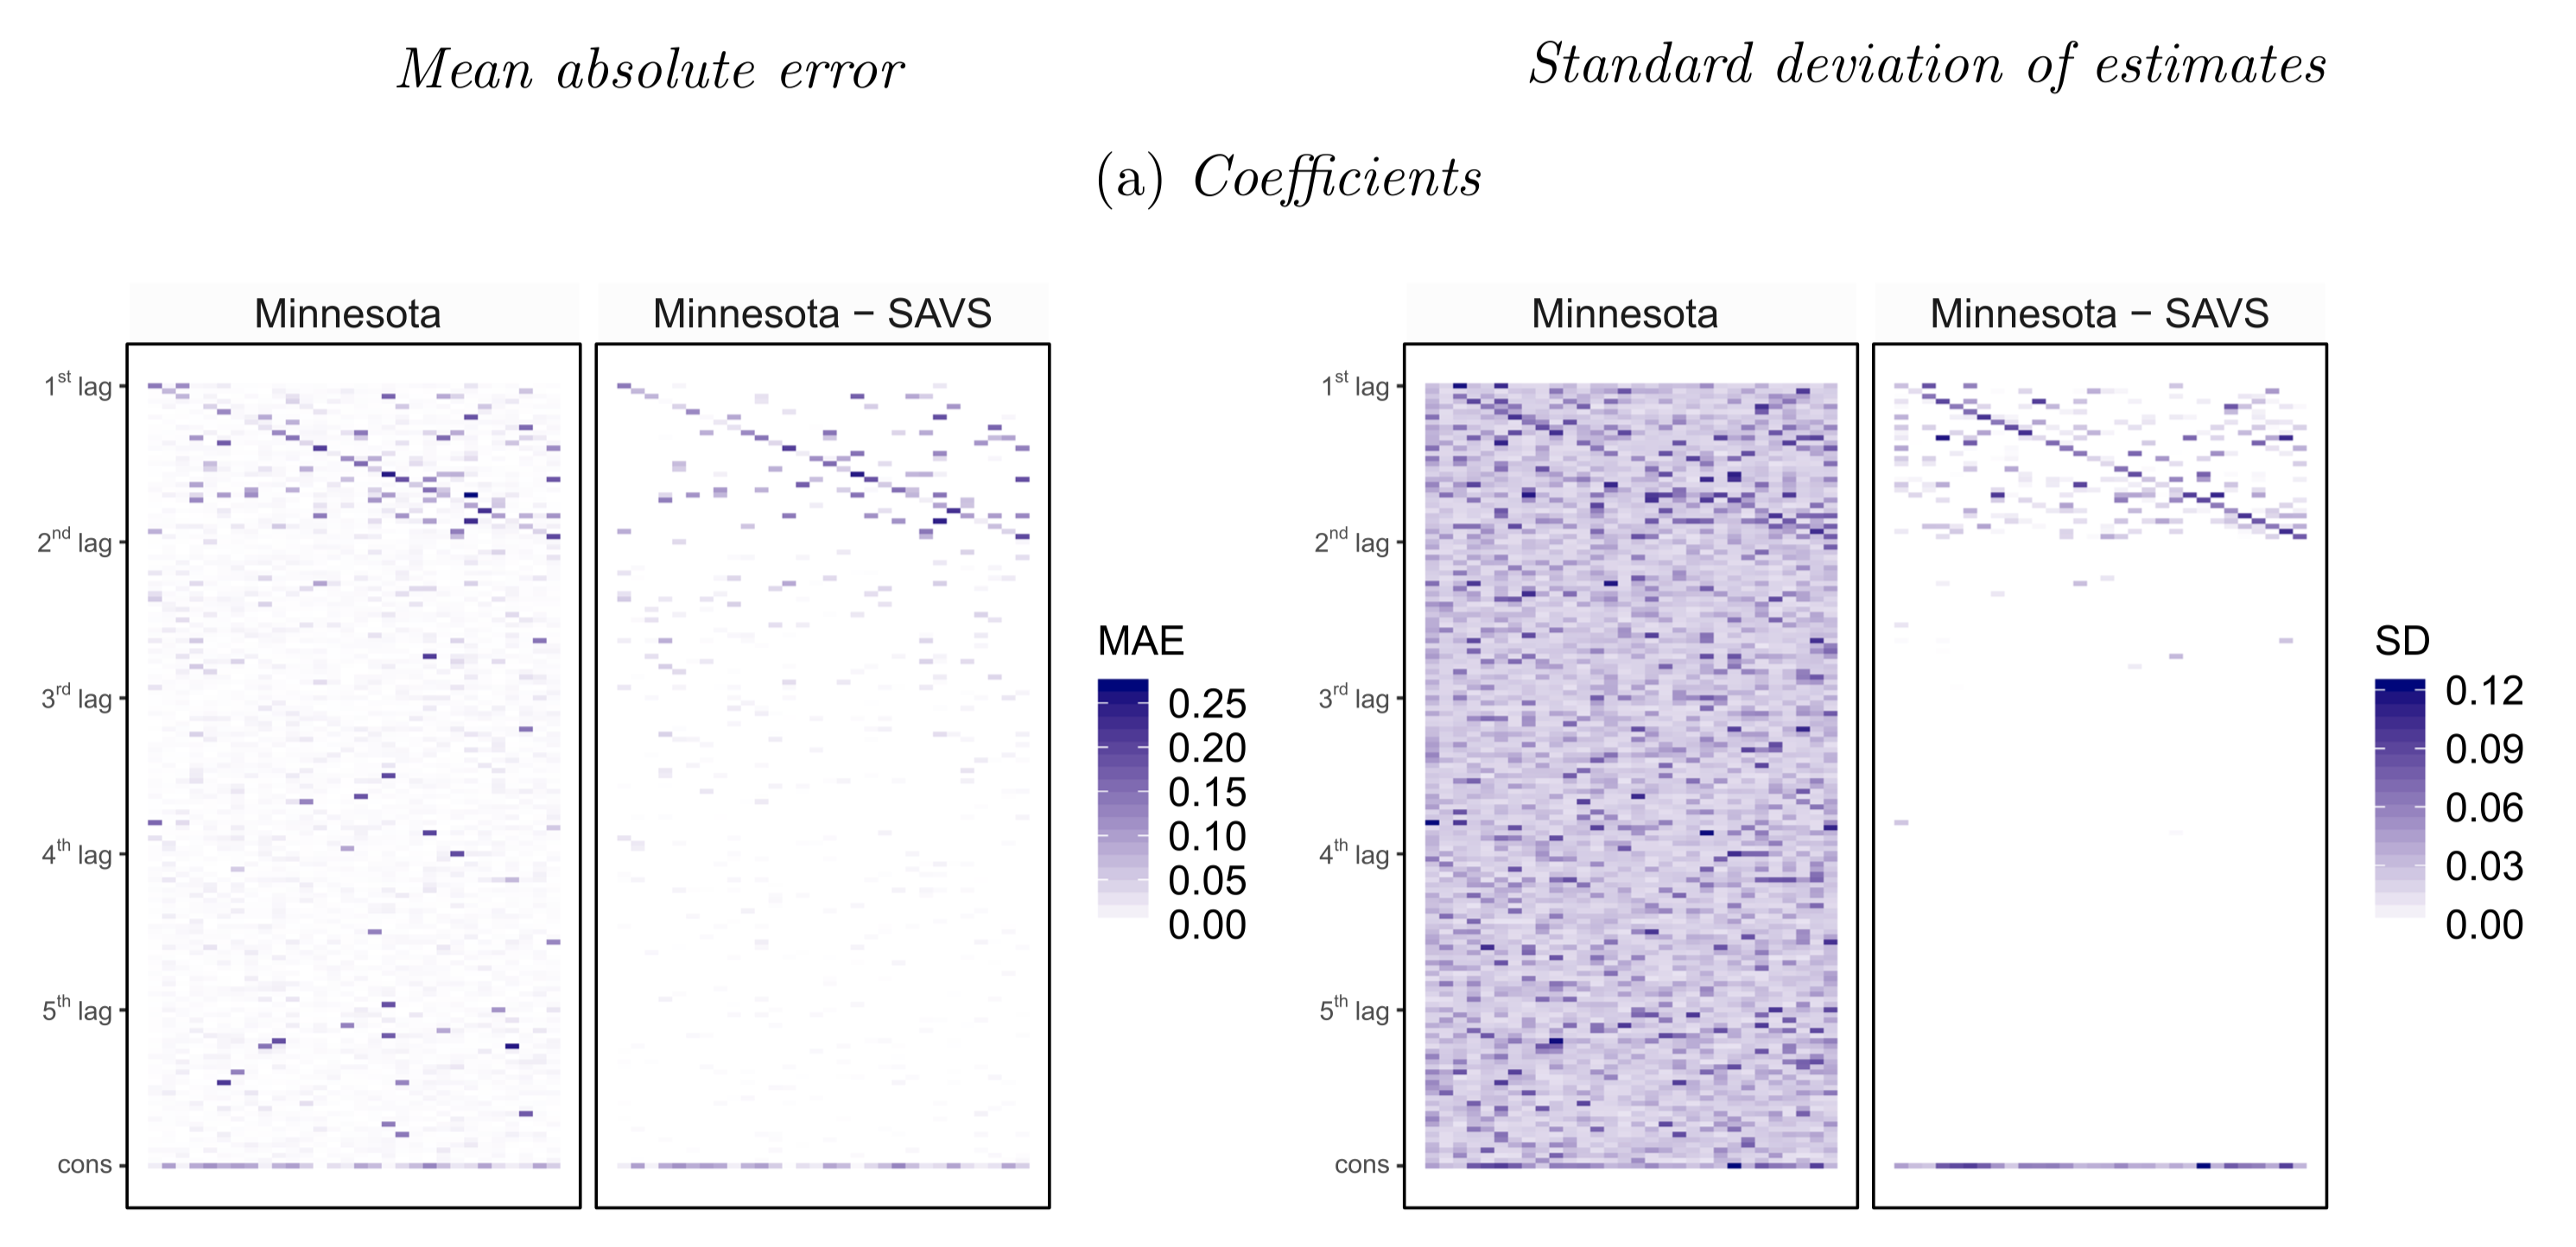
\includegraphics[width=1\textwidth]{plots/sparsity_coefficients.png}
        \caption{Sparsity reduces both the coefficients mean absolute error (MAE) and the predictive parameter uncertainty. The MAE is based on the posterior median estimates measured against the true coefficients. See \nameref{sec:appendix} for covariance estimation results.}
        \label{fig:dense_vs_sparse_coefficients}
    \end{figure}
\end{frame}

%---------------------------------------------------------

%---------------------------------------------------------
\section{Model evaluation using a real-world macroeconomic dataset}

\begin{frame}{Design of the forecasting application}
    \begin{itemize}
        \item Quarterly version of the \cite{mccracken_fred-md_2015} dataset
            \begin{itemize}
                \item Spans U.S. macroeconomic data from 1959:Q1 until 2018:Q4
                \item Target variables: Output (GDPC1), consumer price inflation (CPIAUCSL) and Federal Funds Rate (FEDFUNDS)
                \item Large VAR (\textbf{L-VAR}): VAR(5) with $m = 165$ macroeconomic financial variables
            \end{itemize}
        \item Quarterly recursive forecasting design:
            \begin{itemize}
                \item Initial training period: 1959:Q1 to 1989:Q4 (first 30 years)
                \item Estimation period: $h$-step-ahead predictive distribution for $h \in \{ 1 , 4 , 8 \}$
            \end{itemize}
        \item Evaluation:
            \begin{itemize}
                \item Hold-out period: 1990:Q1 to 2018:Q4
                \item Metrics:\footnote{Mathematical formulation in \nameref{sec:appendix}} Root-mean-squared-forecast-error (RMSE), log predictive likelihood (LPL)
            \end{itemize}
        \item Competitive models to the \textbf{L-VAR} model:
            \begin{itemize}
                \item \textbf{S-VAR}: Small VAR with the three target variables only (benchmark model)
                \item \textbf{M-VAR}: Medium VAR with $m = 21$ variables
                \item \textbf{FA-VAR}: Factor-augmented VAR adding three principal components extracted from the remaining quantities to the \textbf{S-VAR}\footcite{banbura_large_2010,koop_forecasting_2013}
            \end{itemize}
    \end{itemize}
\end{frame}

\begin{frame}{Average point- and density forecast performance}
    Overall, there is only mixed evidence that sparsification in a large-scale model improves the average forecast performance in the hold-out set in comparison to non-sparse and/or smaller models.
    
    \begin{itemize}
        \item $h \in \{ 4 , 8 \}$ forecasts benefit from larger information sets (\textbf{L-VAR})
        \item Sparsification works well for longer run forecasts of output and interest rate
        \item Marginal LPL for inflation: Main driver for bad performance of large models
            \begin{itemize}
                \item Well known result in central bank practice that small models perform better for inflation forecasts\footcite{giannone_prior_2015}
            \end{itemize}
    \end{itemize}
    
    However, sparsification only very rarely hurts forecasting performance in a significant manner on average.
\end{frame}

% Detailed point and density performance slides commented out
\iffalse
    \begin{frame}{Point-forecast performance (measured by RMSEs)}
        No model class outperforms other model classes significantly over all forecast horizons.
        \begin{itemize}
            \item $h \in \{ 4 , 8 \}$ forecasts benefit from larger information sets (\textbf{L-VAR}).
            \item Sparsification works well for longer run point-forecasts of output and inflation.
                \begin{itemize}
                    \item However, sparsification slightly harms predictive accuracy in many other cases.
                \end{itemize}
        \end{itemize}
        
        \begin{itemize}
            \item[$\rightarrow$] There is mixed evidence that sparsification improves point-forecast accuracy. At the same time, it only very rarely hurts accuracy in a statistically significant manner.
        \end{itemize}
    \end{frame}
    
    \begin{frame}{Density forecast performance (measured by LPLs)}
        One-step-ahead forecasts ($h = 1$):
        \begin{itemize}
            \item Joint LPL: Moderately sparse \textbf{M-VAR} performs best
            \item Marginal LPLs for output and interest rate: \textbf{M-VAR} and \textbf{L-VAR} with moderate sparsification are best or at least competitive
            \item Marginal LPL for inflation: Main driver for bad performance of large models
                \begin{itemize}
                    \item Well known result in central bank practice that small models perform better for inflation forecasts\footcite{giannone_prior_2015}
                \end{itemize}
            \item Too strong sparsification hurts density forecast accuracy
                \begin{itemize}
                    \item The predictive density is too narrow meaning that capturing outliers is difficult
                \end{itemize}
        \end{itemize}
        
        Multi-step-ahead forecasts ($h \in \{ 4 , 8 \}$):
        \begin{itemize}
            \item Joint LPL: Similar results like for $h = 1$
            \item Marginal LPLs for output and interest rate: Sparse \textbf{L-VAR} performs best
        \end{itemize}
        
        \begin{itemize}
            \item[$\rightarrow$] The \textbf{L-VAR} model class with moderate to strong sparsification outperforms most other models for output and interest rate.
            \item[$\rightarrow$] Smaller VARs perform better for inflation forecasts.
        \end{itemize}
    \end{frame}
\fi

\begin{frame}{Density forecast performance over time I}
    \begin{figure}
        \centering
        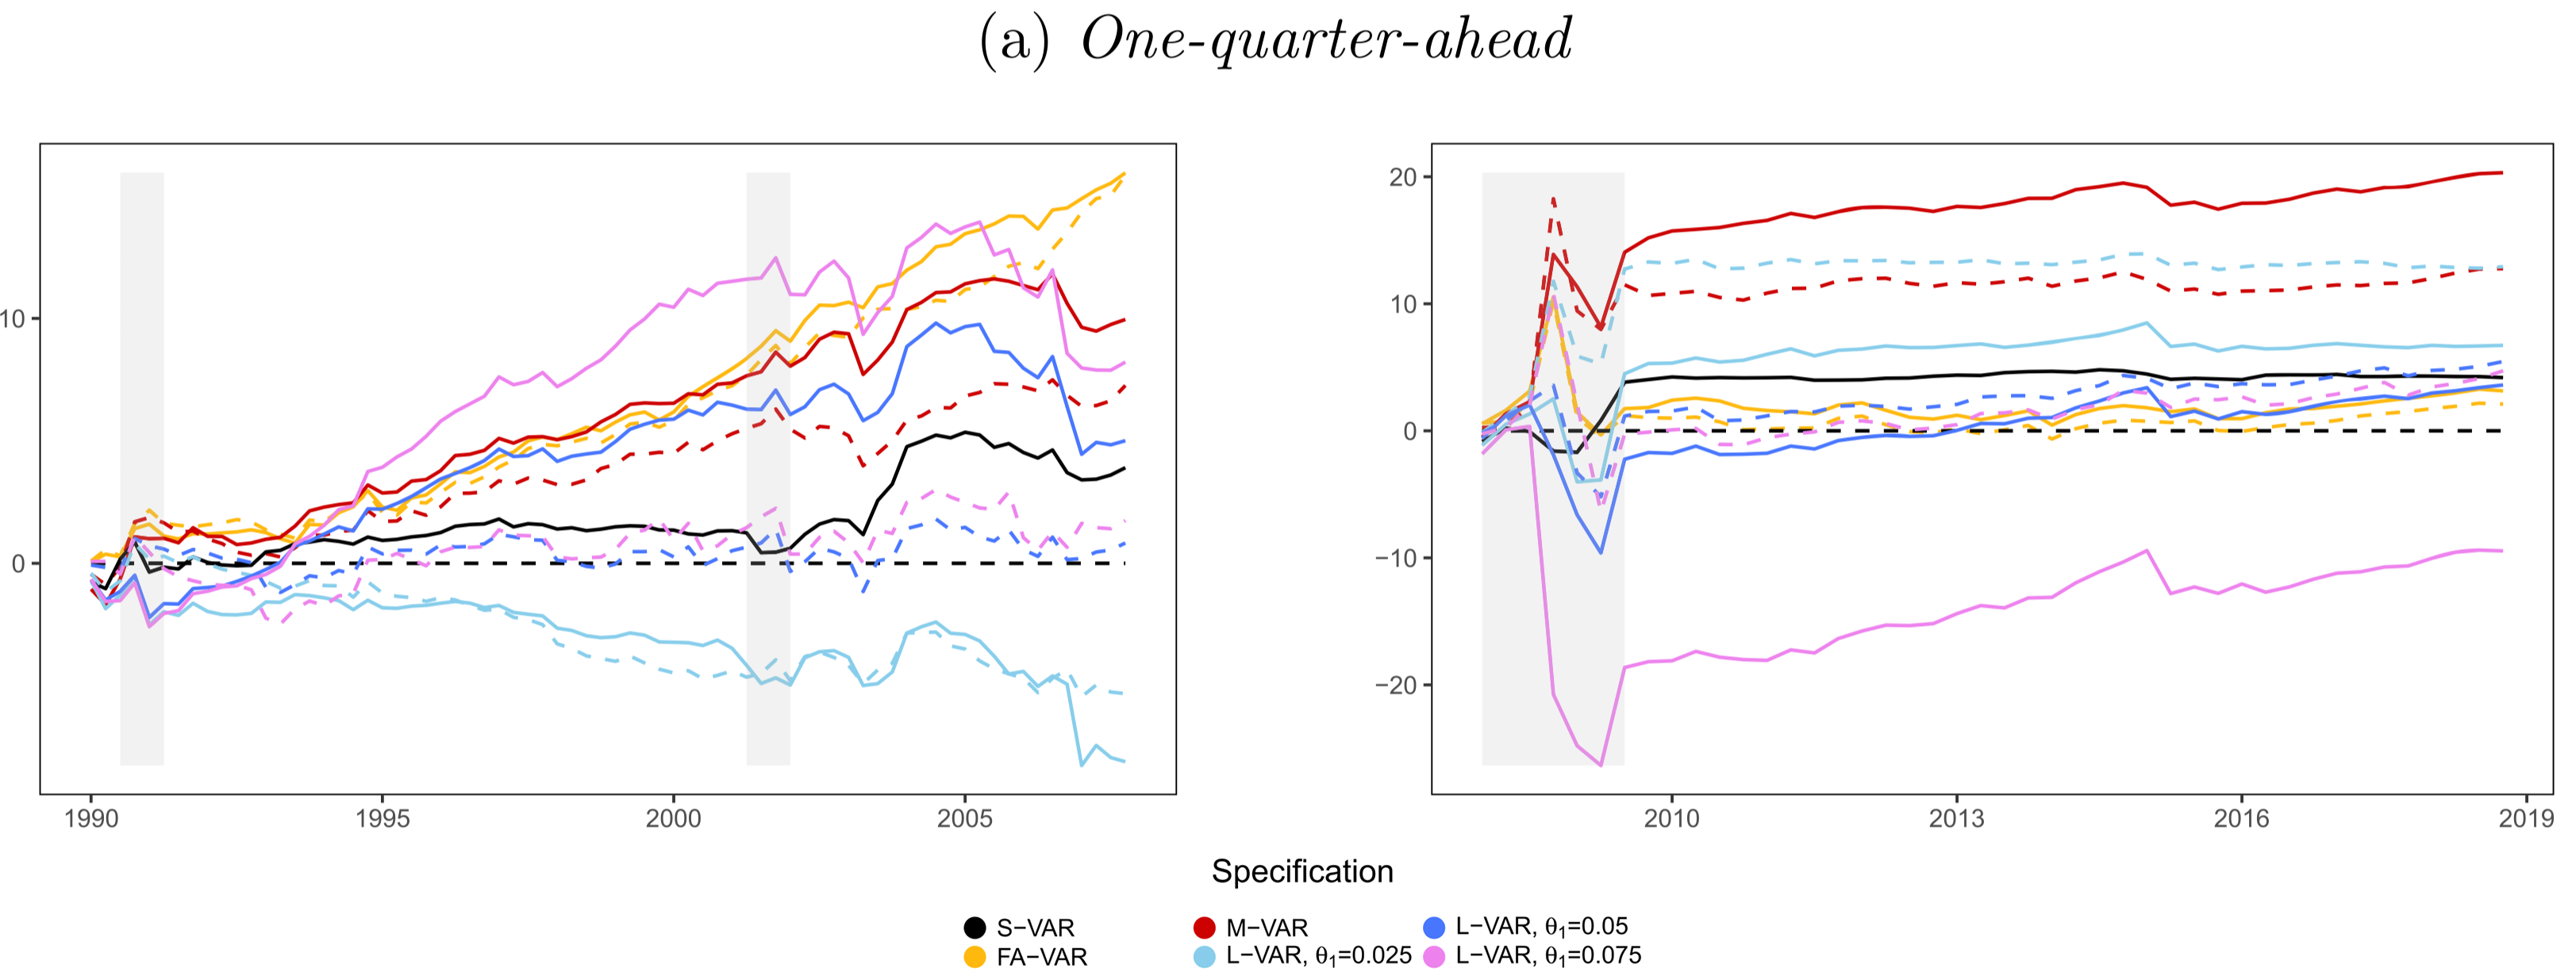
\includegraphics[width=\textwidth]{plots/lpl_one_quarter_ahead.png}
        \caption{Before the financial crisis (left plot) the one-quarter-ahead forecasts of the sparsified large-scale models as measured by the joint cumulative LPLs are very competitive and sometimes better in comparison to the smaller and non-sparsified models. This behavior is reversed during the shock due to the financial crisis (right plot) in 2008. However, the performance increases again after the end of the financial crisis.}
        \label{fig:lpl_one_quarter_ahead}
    \end{figure}
    
    \scriptsize Dashed lines indicate non-sparse models. Solid lines depict the best sparsified model of the class. Smaller $\theta_1$ values put more weight on shrinkage.
\end{frame}

\begin{frame}{Density forecast performance over time II}
    \begin{figure}
        \centering
        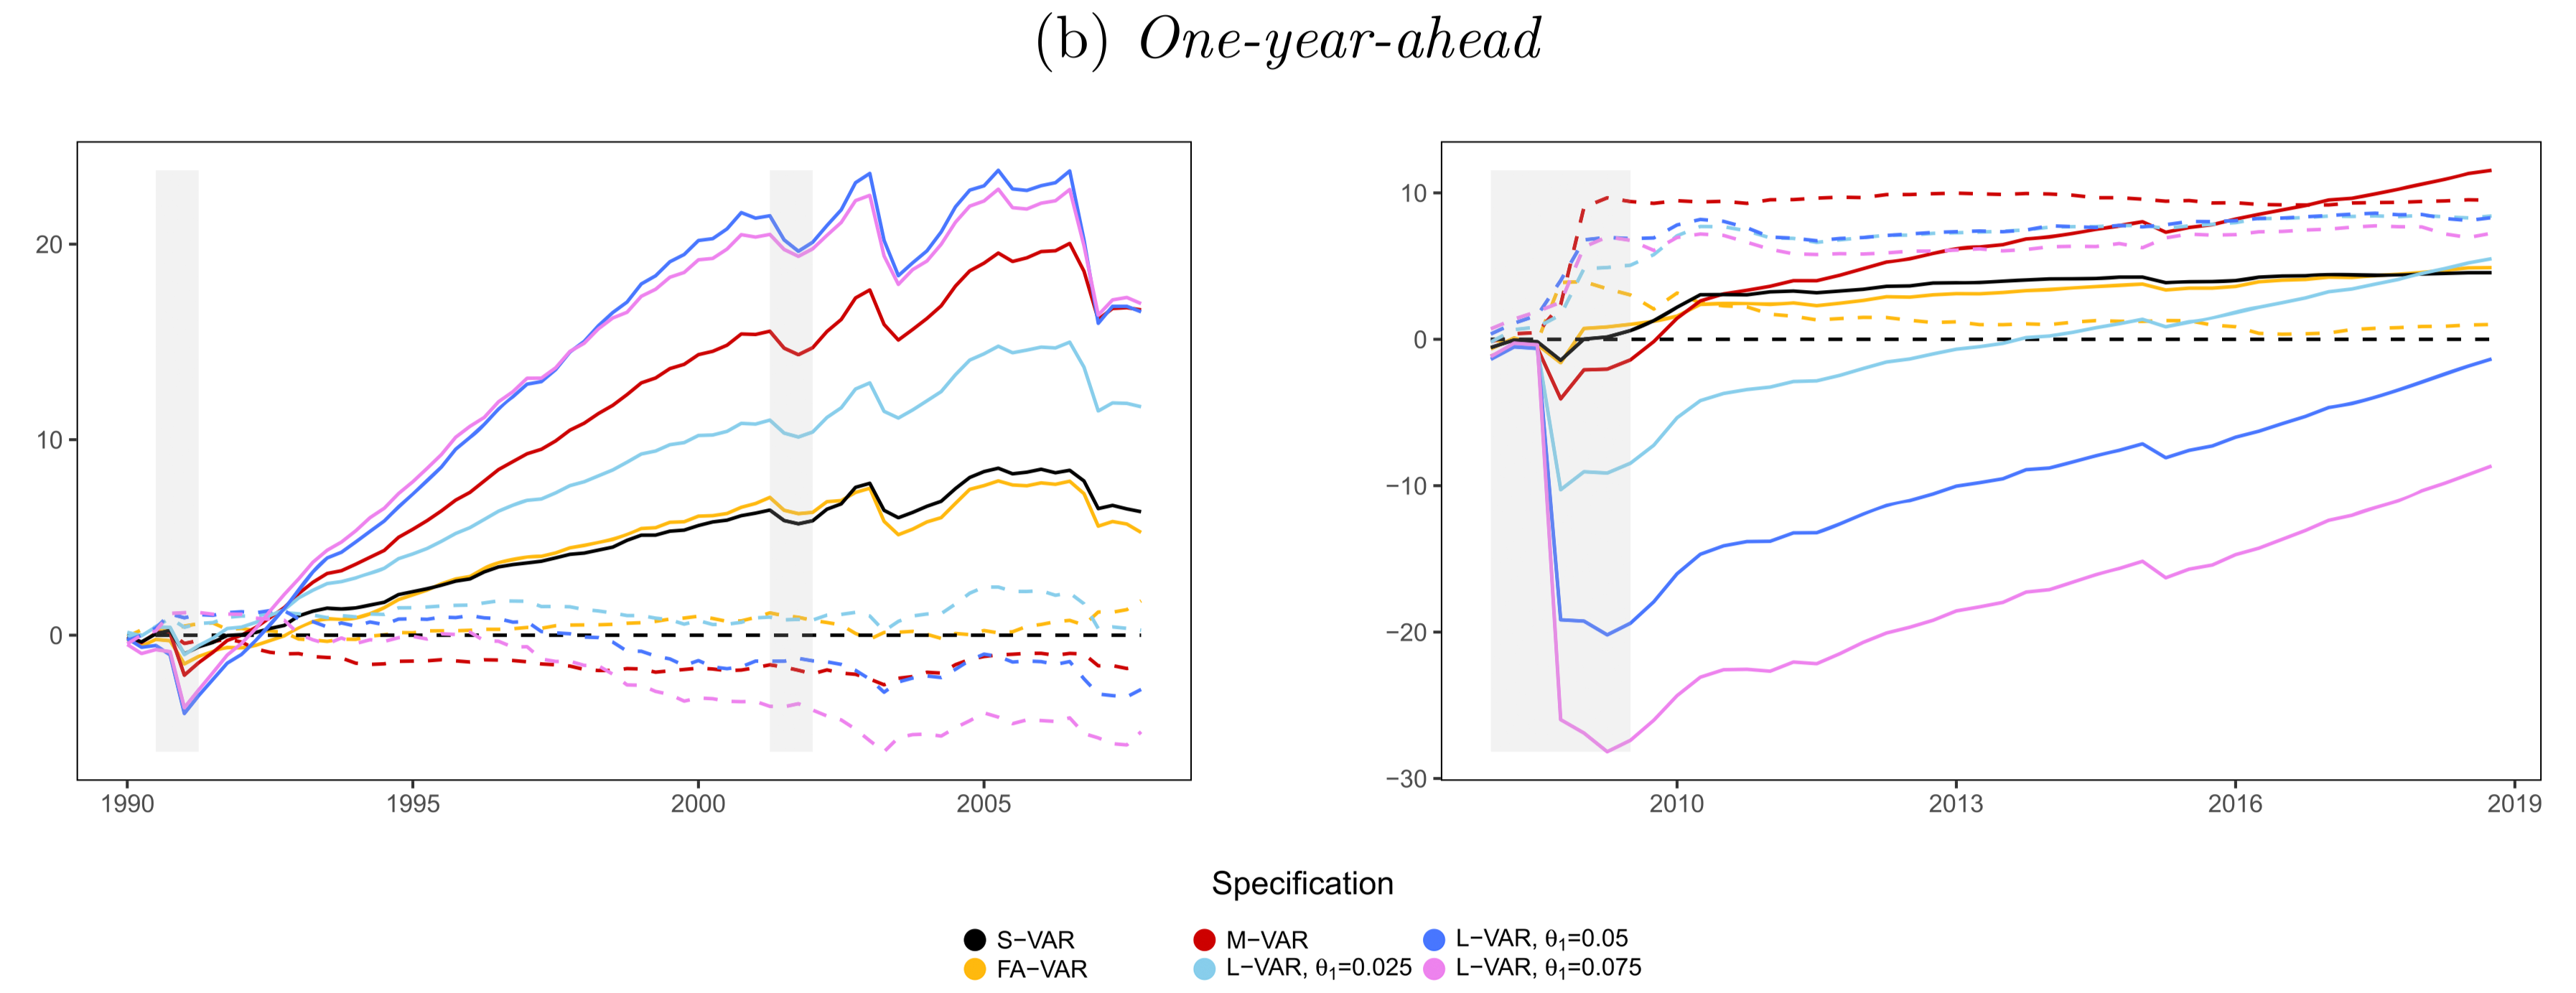
\includegraphics[width=\textwidth]{plots/lpl_one_year_ahead.png}
        \caption{Before the financial crisis (left plot) the one-year-ahead forecasts of the sparsified large-scale models as measured by the joint cumulative LPLs are significantly superior to the smaller and non-sparsified models. This behavior is reversed during the shock due to the financial crisis (right plot) in 2008. However, the performance increases steeply after the end of the financial crisis.}
        \label{fig:lpl_one_year_ahead}
    \end{figure}
    
    \scriptsize Dashed lines indicate non-sparse models. Solid lines depict the best sparsified model of the class. Smaller $\theta_1$ values put more weight on shrinkage.
\end{frame}
%---------------------------------------------------------

%---------------------------------------------------------
\section{Conclusion}

\begin{frame}{Conclusion}
    \begin{itemize}
        \item Natural conjugate priors allow for direct sampling from the posterior distributions
            \begin{itemize}
                \item This speeds up the process of approximating a sparsified posterior
            \end{itemize}
        \item Shrinkage alone is not enough to reduce predictive uncertainty due to the curse of dimensionality in large-scale VAR models
            \begin{itemize}
                \item Sparsification works well for many cases but has problems in catching outliers (e.g. financial crisis)
            \end{itemize}
        \item The sparsification algorithm is heavy on CPU time even for the natural conjugate prior
            \begin{itemize}
                \item The Paper's results could not be reproduced on a fast desktop PC
            \end{itemize}
    \end{itemize}
\end{frame}
%---------------------------------------------------------

